\section{XMD - XMV integration}

\subsection{QML}

The xMAS model designer has been created in QML. QML is a declarative language
that can be used to quickly design user interfaces. It has a JSON-like syntax
which allows developers to describe visual components and their interactions
in a readable and compact notation. Inside a QML file, JavaScript expressions
and functions can be used. This enables developers to add logic using a familiar
scripting language. Furthermore, QML provides a C++ API to connect the user
interface with back-end C++ libraries.

\subsection{User interface}

The applications user interface is composed of multiple qml files. They are split
in two folders. In folder 'uicontrols', the QML files that make up the user interface
controls like the toolbar, console and dialogs are placed. Folder 'xobjects'
contains QML files that are used to draw the xMAS components on the designer
canvas. At the root of the user interface definition is mainWindow.qml.

\paragraph{}
In addition to the qml files, some JavaScript functions are placed in separate
.js files. This has been done for organizational reasons. Small JavaScript fragments
are placed inside the qml files. Larger fragments and fragments that contain logic
are placed inside .js files. This division keeps both files uncluttered. The same
.js file can be imported in multiple qml files, so reuse of code is improved as well.

\subsection{C++ integration}
QML objects can interact with each other by either directly accessing their property
values or through the signal/slot mechanism. Interaction between QML and C++
classes is slightly more complicated. The application uses two methods provided
by QML to integrate QML and C++ objects.

\subsubsection{QML Context property}
Each QML application operates in a certain QML context. The QML context stores
properties that are available throughout all QML code. C++ classes can be exposed
to the QML world by setting a C++ object instance as the value of a property
on the QML context.
XMD uses context properties to provide access to three C++ classes:

\begin{itemize}
 \item \textbf{datacontrol} (of class DataControl) to provide access to the
 underlying xMAS data model
 \item \textbf{plugincontrol} (of class PluginControl) to provide access to
 the plugins that manage starting and stopping of verification tools
 \item \textbf{util} (of class Util) to provide utility functions
\end{itemize}

\begin{figure}
    \includegraphics[width=\textwidth]{qml3}
    \caption{Registering a QML context property}
\end{figure}

\paragraph{QML Documentation}
More information on context properties is available at:
\url{http://doc.qt.io/qt-5/qtqml-cppintegration-contextproperties.html}


\subsubsection{Embedding C++ classes in QML}

QML applications can also be extended with C++ code by registering C++ classes
with the QML type system. Any C++ class that derives from QObject can be used
in this way. Registering the class to QML not only allows access to the properties,
methods and signals of an object. Additionally, QML code can directly instantiate
new objects of the registered classes (see figure~\ref{fig:register-qml}).

\begin{figure}
    \includegraphics[width=\textwidth]{qml1}
    \includegraphics[width=\textwidth]{qml2}
    \caption{Exposing a C++ class to QML}
    \label{fig:register-qml}
\end{figure}

\paragraph{Usage}XMD registers four C++ classes to the QML type system. These classes
are \textbf{Channel}, \textbf{XPort}\footnote{This class has been named XPort to
avoid confusion with the Port class defined in the xMAS data model}, \textbf{Network}
and \textbf{Component}. The definitions of each of the four classes is split in
three files. The .h and .cpp files contain normal C++ header and source files of
the classes. Furthermore, each class has a QML file which contains additional
QML code (figure~\ref{fig:qml-cpp-classes}). All three files belong to the same
class. The QML type system binds the C++ code and the QML code together to form a
single class definition. Note that a class can have different names in C++ code
and QML code, e.g. Channel (C++) vs. XChannel (QML). Registration of types is
done by a call to qmlRegisterType, figure~\ref{fig:register-qml} shows an example.

\paragraph{QML Documentation}
More information is available at:
\url{http://doc.qt.io/qt-5/qtqml-tutorials-extending-qml-example.html}


\begin{figure}
    \centering
    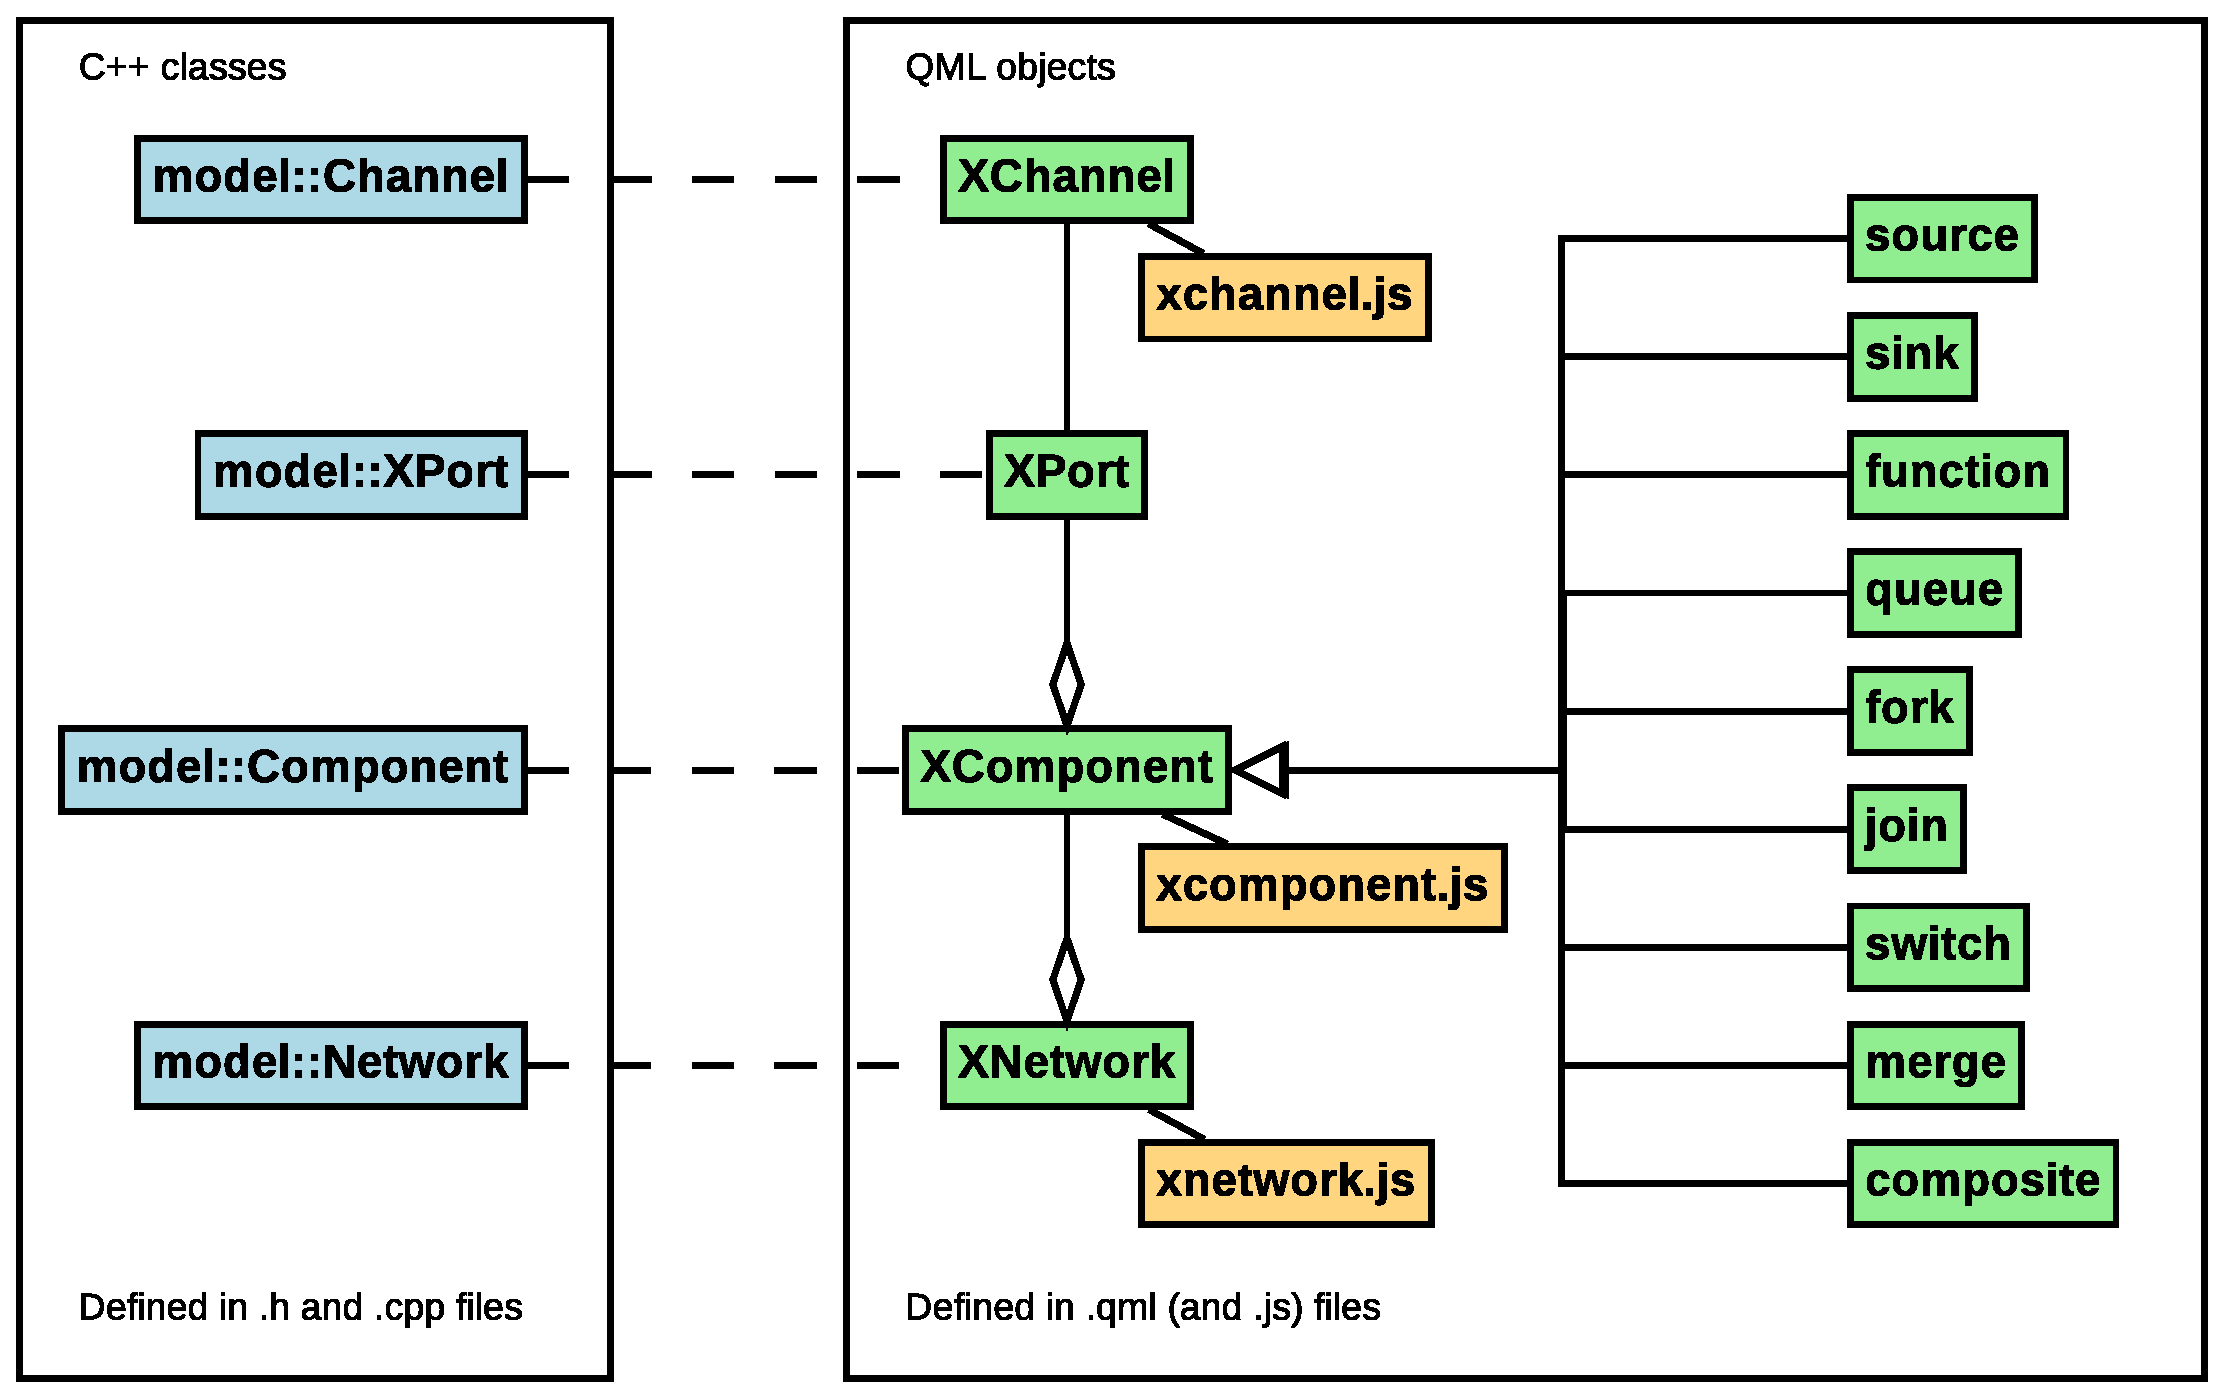
\includegraphics[width=0.8\textwidth]{qml-cpp-classes}
    \caption{Qml / C++ integration of XMD classes}
    \label{fig:qml-cpp-classes}
\end{figure}


\subsubsection{Interaction xmd / datamodel classes}

Figure~\ref{fig:xmd-xmv-integration} shows the relationship between the classes of
xmd and the the datamodel. The bottom part contains the model classes, which are
shared by both xmv and xmd. The equivalant (QML) classes that make up the view are
located in the upper part. The xmd classes XPort and Component do not directly
access the Port and XMASComponent classes of the datamodel. Manipulation of the
datamodel always involves class DataControl. This class has access to the project,
its root network and the components and ports of the model under construction.

\begin{figure}[ht]
    \includegraphics[width=\textwidth]{xmd-xmv-integration}
    \caption{Integration of xmd and xmv datamodel}
    \label{fig:xmd-xmv-integration}
\end{figure}


\newpage
\subsubsection{Architecture}

\begin{figure}[ht]
    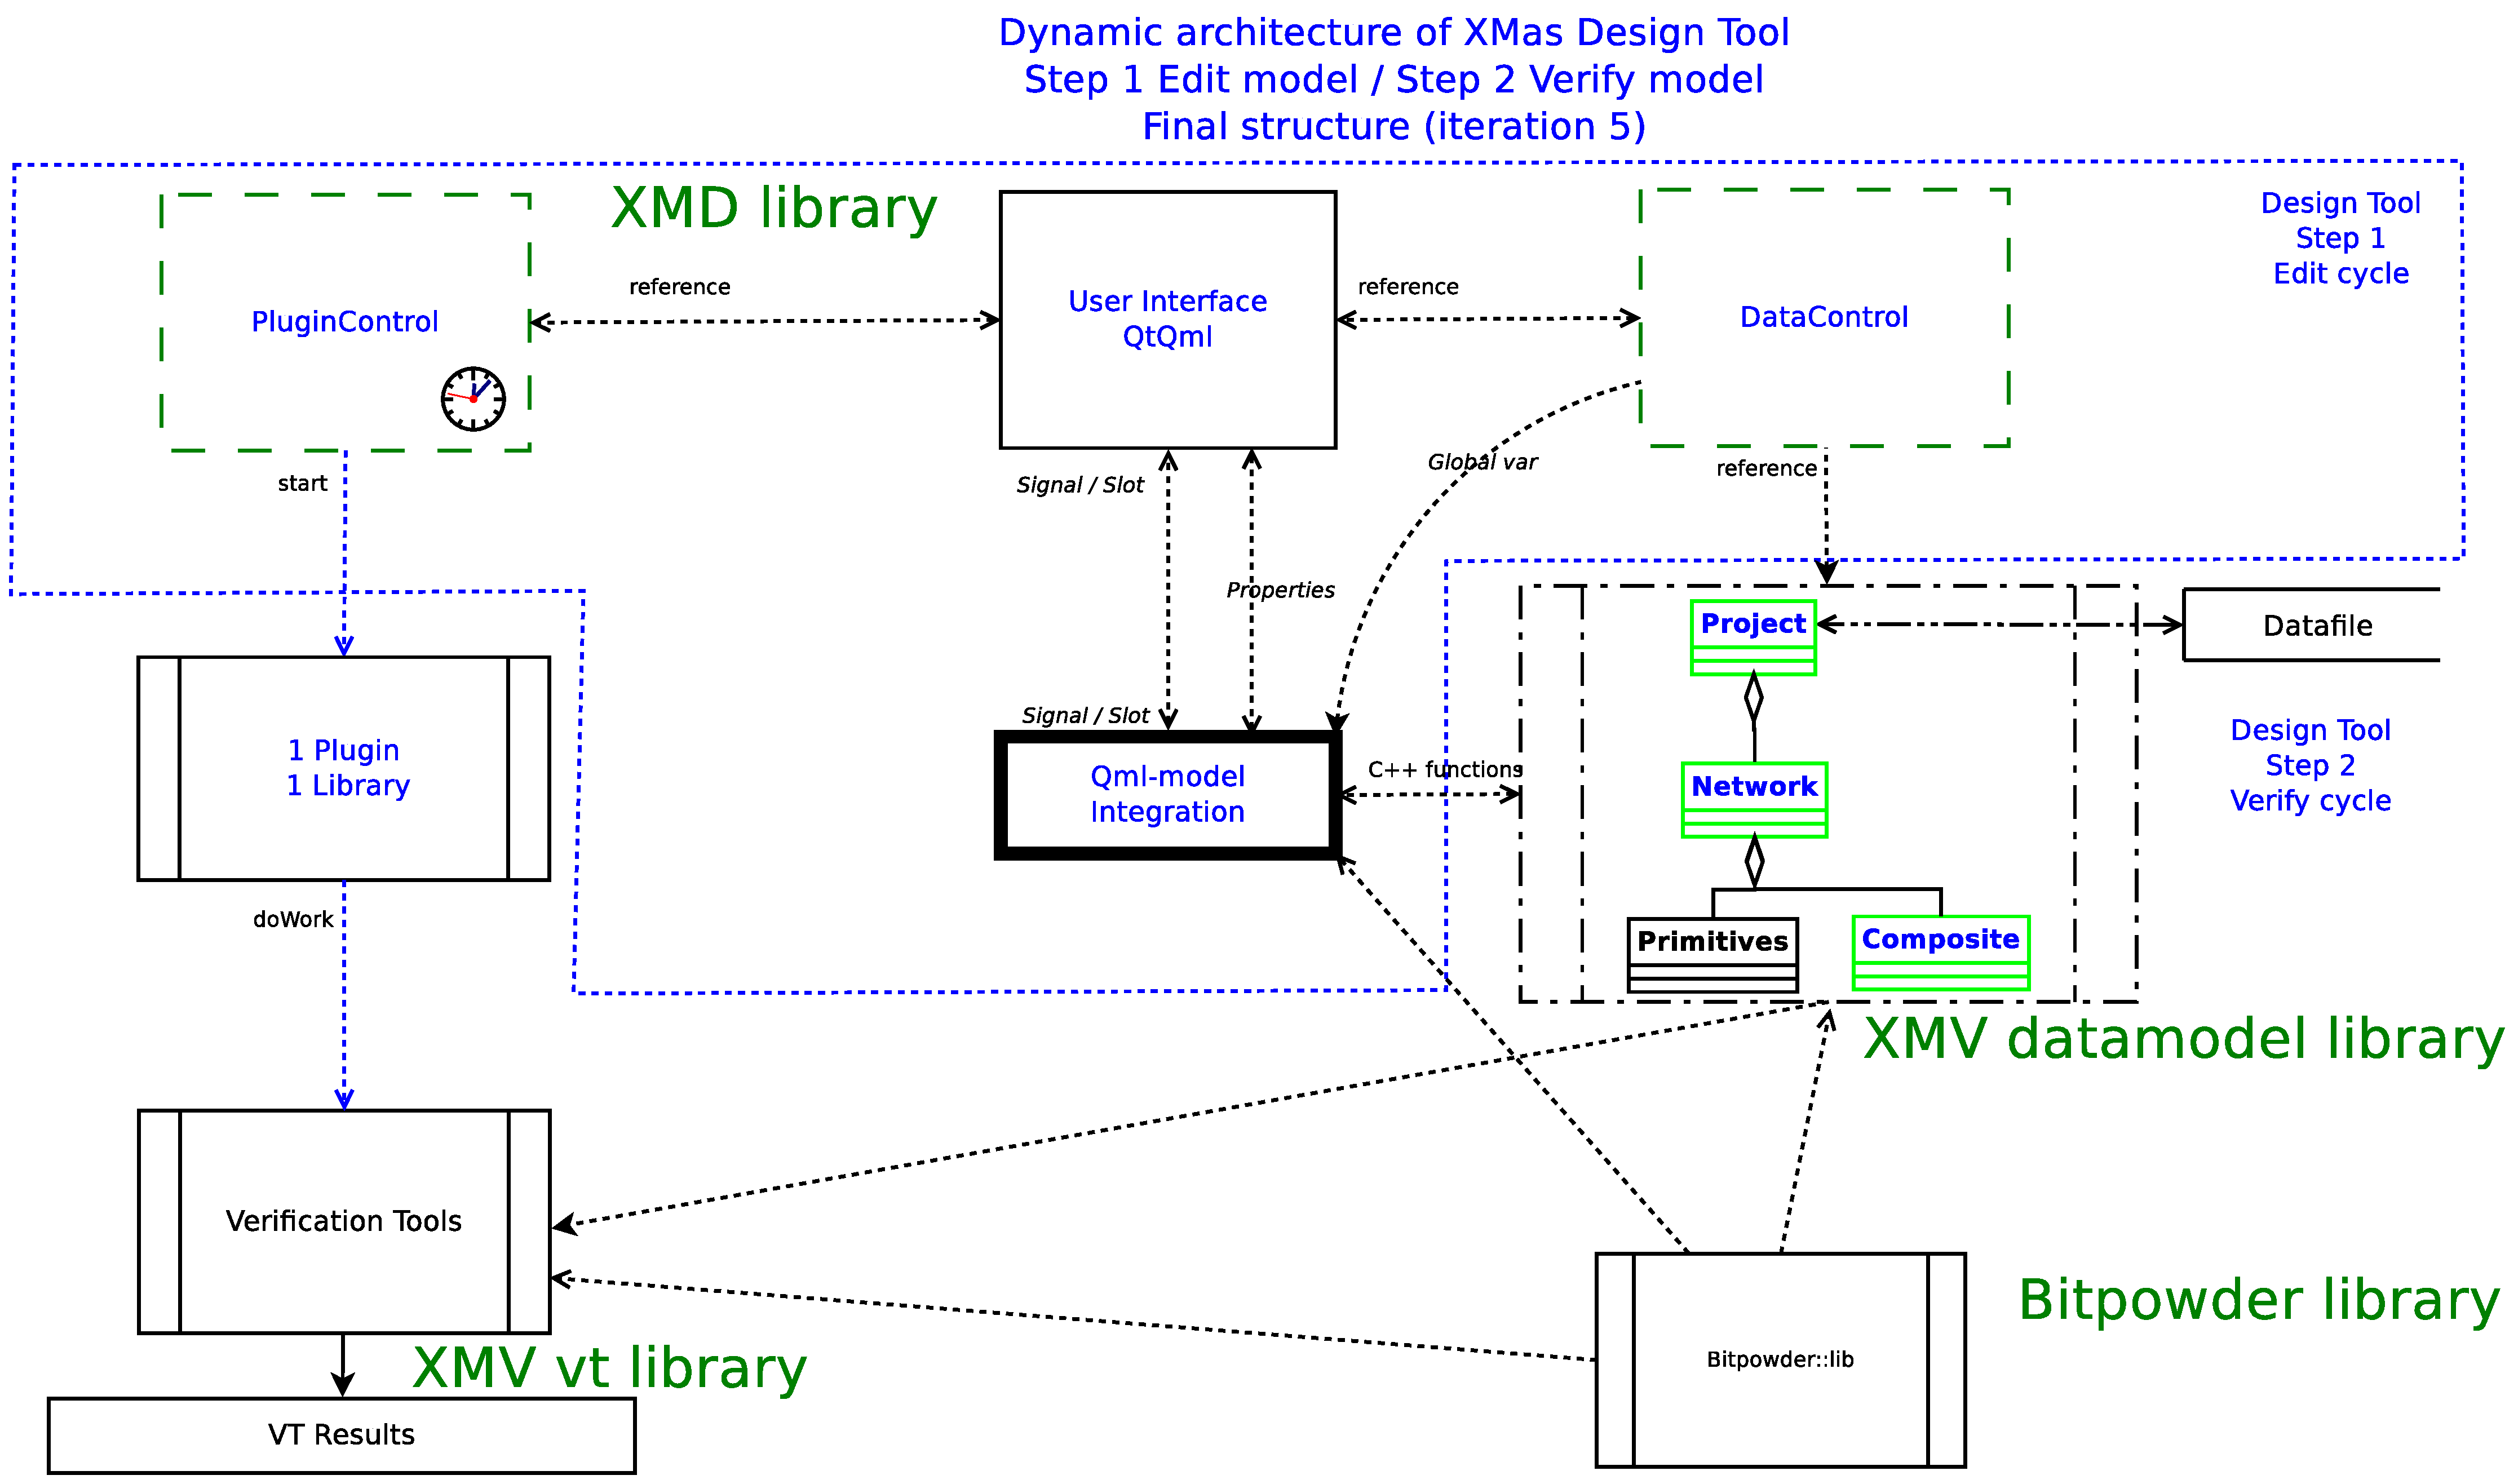
\includegraphics[width=\textwidth]{1c-architecture-dynamic-2}
    \caption{Global system architecture}
\end{figure}
